\chapter{System Design}
\label{chapter:SystemDesign}
%\TODO{In this part we will introduce the software design of both server and client side. }

\begin{figure}[htb]
	\centering
	
	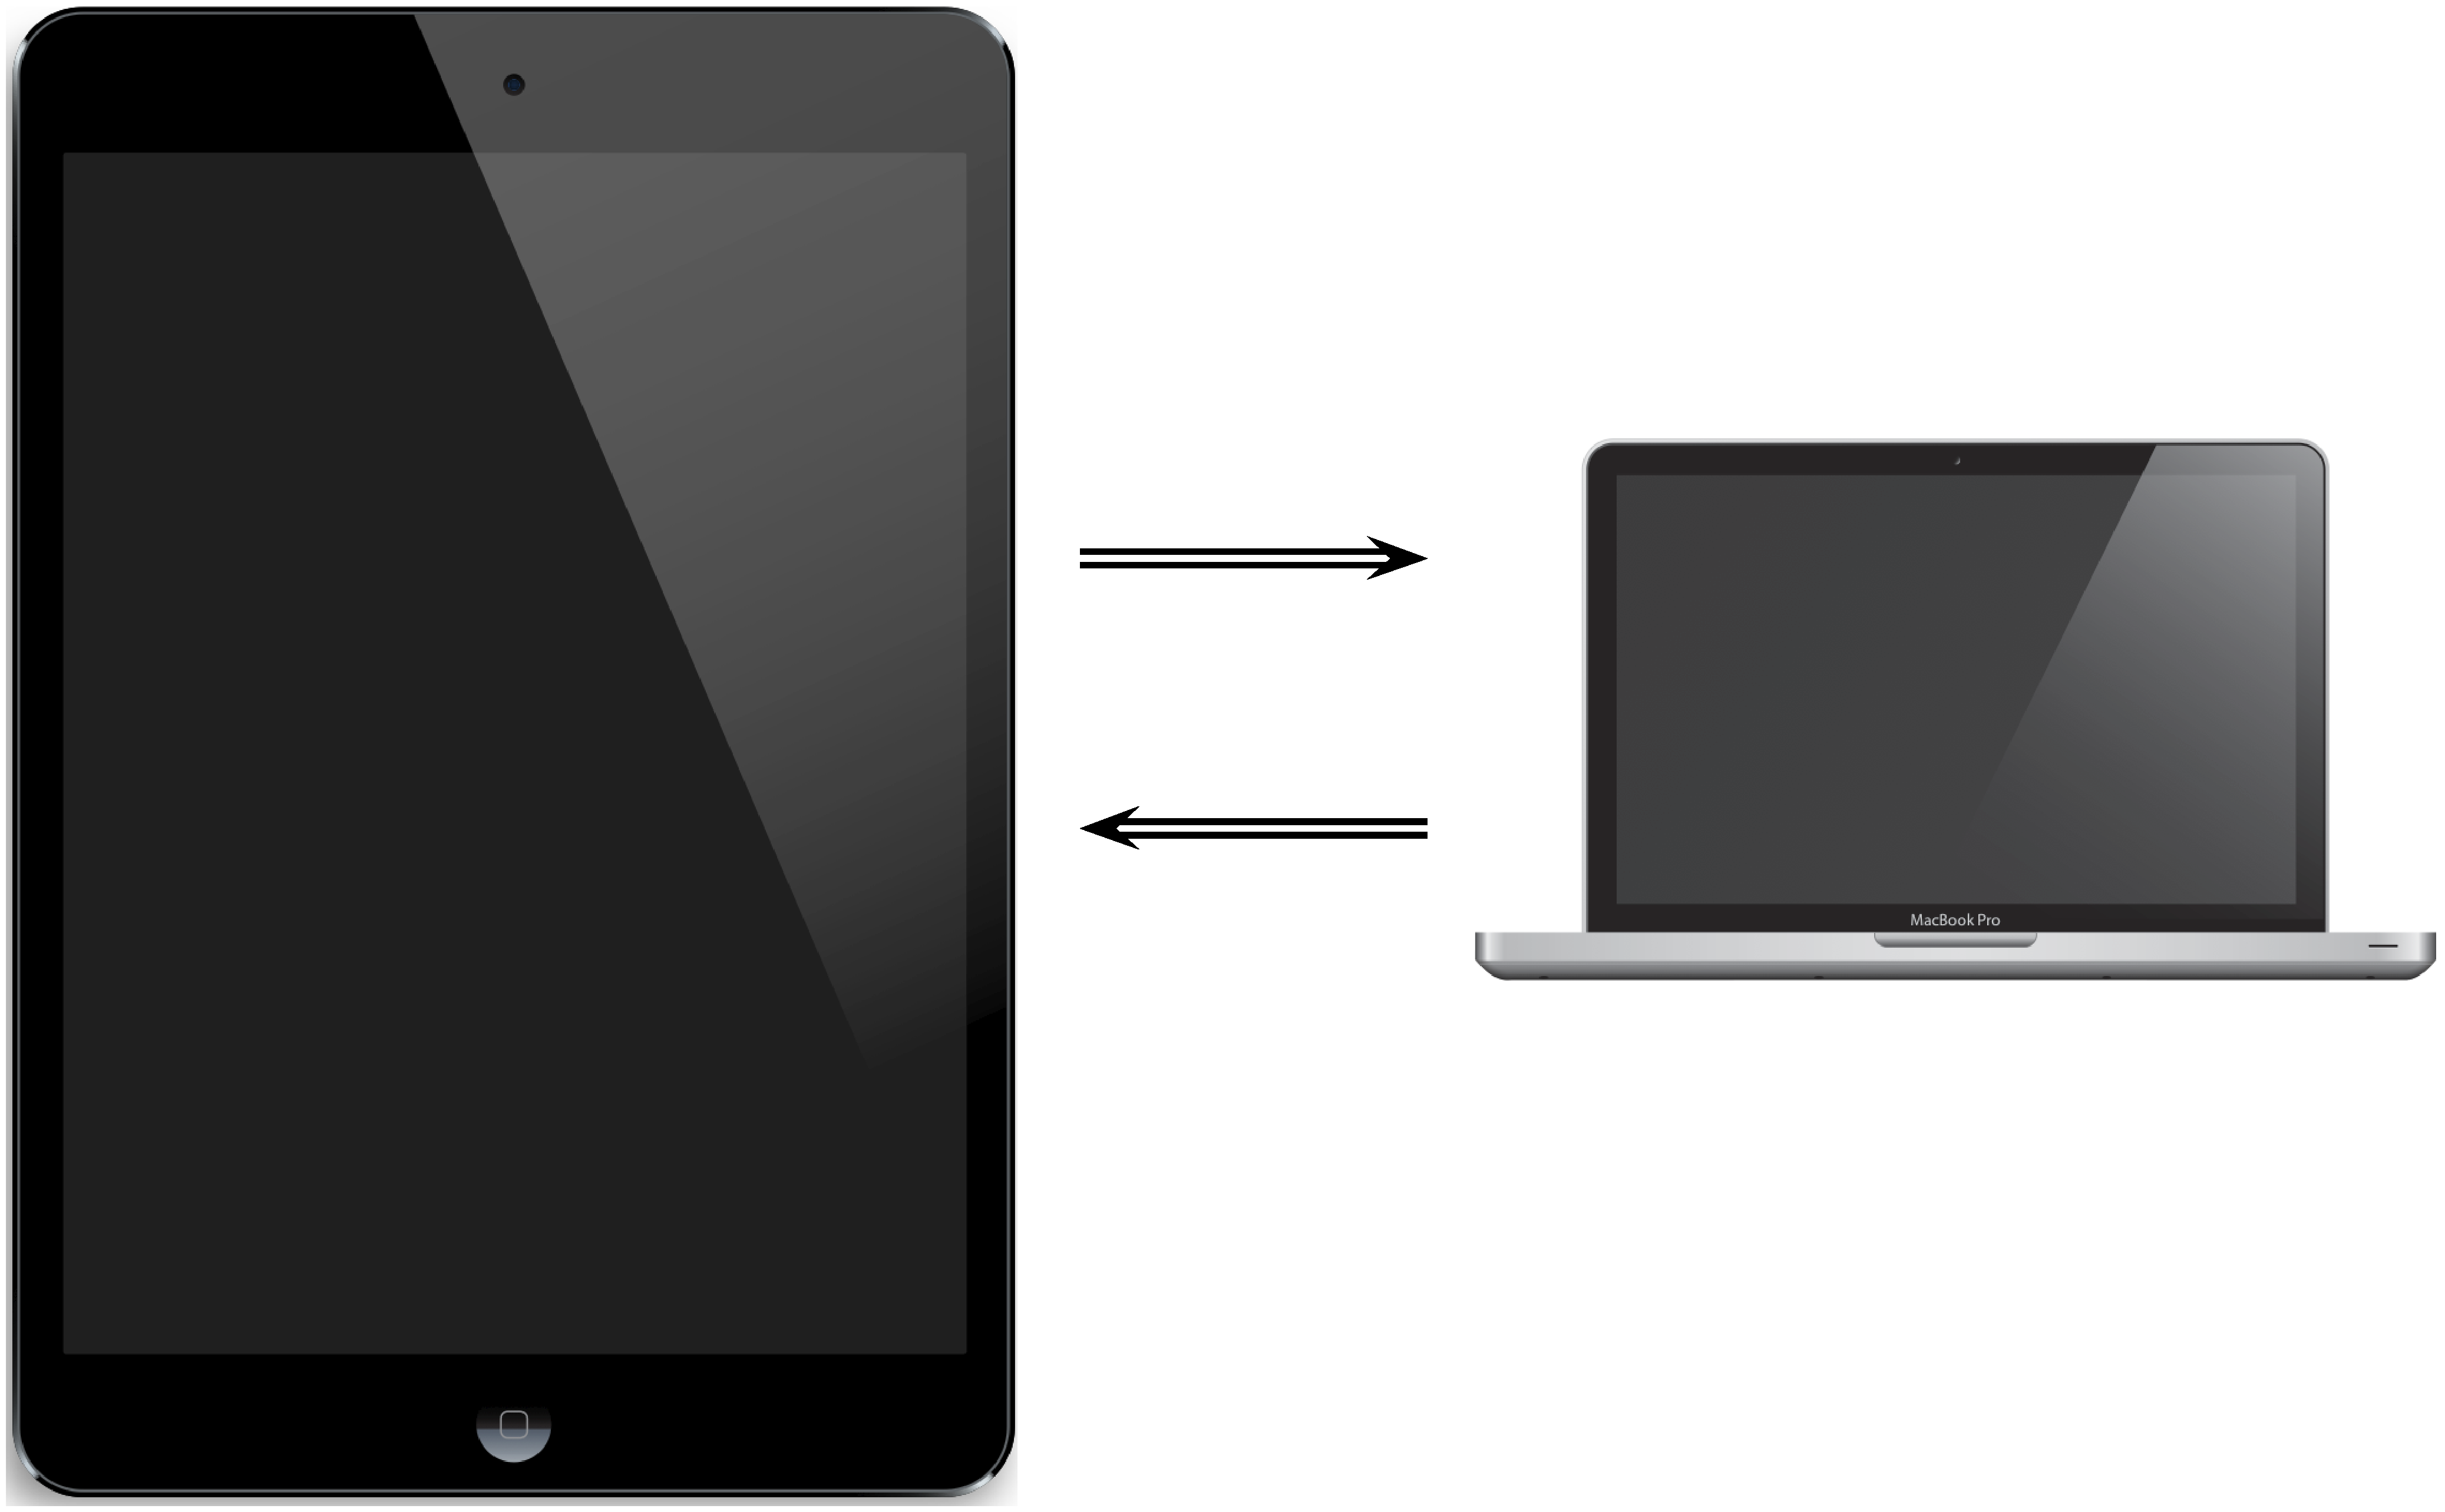
\includegraphics[scale=0.2]{graphs/images/client_server_illu.pdf}
	\caption{Application's Client and Server Architecture}
	\label{fig:clientserver}

\end{figure}
The main contribution of this thesis the view-dependent geometry streaming application implemented on mobile device. As stated in the previous chapters, our streaming application can be divided into to parts: client and server. (see \FG{fig:clientserver}) The client application is developed in Objective-C and deployed on a the iOS system. And the server part of the application is running on a an ordinary PC. In this chapter, software design detail of the both server-side and client-side will be described. \\

This chapter is organized as follows: First in \SC{section:serverdesign} we describe the software design of our geometry streaming server. We will focus on the software architecture of the server application. Then in \SC{section:clientdesign} we describe the software design of our geometry streaming client on iOS. And we will illustrate the implementation details in Chapter~\ref{chapter:SystemImplementation}.

\section{Server-side Design}
\label{section:serverdesign}

\begin{figure}[htb]
	\centering
	
	\begin{pdfpic}
	\psset{unit=0.90cm}
	\begin{pspicture}
	\psframe[linewidth=0.1,framearc=0.05,dimen=outer,shadow=true,shadowangle=-45.0,fillstyle=solid](16.0,4.4)(0.0,-4.4)
\psline[linewidth=0.2cm,arrowsize=0.073cm 2.6,arrowlength=0.6,arrowinset=0.3]{<-}(13.8,2.4)(13.8,-1.6)
\psline[linewidth=0.2cm,arrowsize=0.073cm 2.0,arrowlength=0.6,arrowinset=0.3]{<-}(6.4,2.4)(6.4,-1.6)
\psframe[linewidth=0.1,framearc=0.1,dimen=outer,shadow=true,shadowangle=-45.0,fillstyle=solid](7.8,1.8)(0.6,-0.8)
\psframe[linewidth=0.06,framearc=0.1,dimen=outer,shadow=true,shadowangle=-45.0,fillstyle=solid](3.0,1.0)(1.0,-0.4)
\psframe[linewidth=0.06,framearc=0.1,dimen=outer,shadow=true,shadowangle=-45.0,fillstyle=solid](5.2,1.0)(3.2,-0.4)
\psframe[linewidth=0.06,framearc=0.1,dimen=outer,shadow=true,shadowangle=-45.0,fillstyle=solid](7.4,1.0)(5.4,-0.4)
\usefont{T1}{ppl}{m}{n}
\rput(4.2684035,1.32){\small Network}
\usefont{T1}{ppl}{m}{n}
\rput(1.8684033,0.52){\small Network}
\usefont{T1}{ppl}{m}{n}
\rput(1.8211719,0.12){\small Protocol}
\usefont{T1}{ppl}{m}{n}
\rput(3.8788085,0.72){\small Socket}
\usefont{T1}{ppl}{m}{n}
\rput(4.140884,0.32){\small Transmitt}
\usefont{T1}{ppl}{m}{n}
\rput(4.1679397,-0.08){\small Controller}
\usefont{T1}{ppl}{m}{n}
\rput(6.042378,0.52){\small Vsplit}
\usefont{T1}{ppl}{m}{n}
\rput(6.356079,0.12){\small streaming}
\usefont{T1}{ppl}{m}{n}
\rput(7.8651757,3.605){\LARGE Progressive Mesh Server}
\psframe[linewidth=0.1,framearc=0.5,dimen=outer,shadow=true,shadowangle=-45.0,fillstyle=solid](15.8,3.2)(0.2,2.4)
\psframe[linewidth=0.1,framearc=0.1,dimen=outer,shadow=true,shadowangle=-45.0,fillstyle=solid](7.8,-1.4)(0.6,-3.8)
\psframe[linewidth=0.1,framearc=0.1,dimen=outer,shadow=true,shadowangle=-45.0,fillstyle=solid](15.4,1.8)(8.2,-0.8)
\psframe[linewidth=0.06,framearc=0.1,dimen=outer,shadow=true,shadowangle=-45.0,fillstyle=solid](4.0,-2.2)(1.0,-3.4)
\psframe[linewidth=0.06,framearc=0.1,dimen=outer,shadow=true,shadowangle=-45.0,fillstyle=solid](10.6,1.0)(8.6,-0.4)
\usefont{T1}{ppl}{m}{n}
\rput(4.04562,-1.88){\small Server Metadata}
\usefont{T1}{ppl}{m}{n}
\rput(11.9696,1.32){\small PM Manager}
\usefont{T1}{ppl}{m}{n}
\rput(2.4318457,-2.68){\small Server Info}
\psframe[linewidth=0.06,framearc=0.1,dimen=outer,shadow=true,shadowangle=-45.0,fillstyle=solid](12.8,1.0)(10.8,-0.4)
\psframe[linewidth=0.06,framearc=0.1,dimen=outer,shadow=true,shadowangle=-45.0,fillstyle=solid](15.0,1.0)(13.0,-0.4)
\usefont{T1}{ppl}{m}{n}
\rput(9.052651,0.52){\small PM}
\usefont{T1}{ppl}{m}{n}
\rput(9.6076565,0.12){\small Repository}
\usefont{T1}{ppl}{m}{n}
\rput(11.252651,0.52){\small PM}
\usefont{T1}{ppl}{m}{n}
\rput(11.5207615,0.12){\small Loader}
\usefont{T1}{ppl}{m}{n}
\rput(13.705142,0.52){\small VDPM}
\usefont{T1}{ppl}{m}{n}
\rput(13.798809,0.12){\small Support}
\psframe[linewidth=0.06,framearc=0.1,dimen=outer,shadow=true,shadowangle=-45.0,fillstyle=solid](7.4,-2.2)(4.4,-3.4)
\usefont{T1}{ppl}{m}{n}
\rput(5.790967,-2.68){\small Model List}
\psframe[linewidth=0.1,framearc=0.1,dimen=outer,shadow=true,shadowangle=-45.0,fillstyle=solid](15.4,-1.4)(8.2,-3.8)
\psframe[linewidth=0.06,framearc=0.1,dimen=outer,shadow=true,shadowangle=-45.0,fillstyle=solid](11.6,-2.2)(8.6,-3.4)
\usefont{T1}{ppl}{m}{n}
\rput(11.706909,-1.88){\small Server Rendering}
\usefont{T1}{ppl}{m}{n}
\rput(9.880346,-2.68){\small Renderer}
\psframe[linewidth=0.06,framearc=0.1,dimen=outer,shadow=true,shadowangle=-45.0,fillstyle=solid](15.0,-2.2)(12.0,-3.4)
\usefont{T1}{ppl}{m}{n}
\rput(13.061553,-2.68){\small Image}
\usefont{T1}{ppl}{m}{n}
\rput(13.497939,-3.08){\small Compressor}
\psline[linewidth=0.2cm,fillcolor=black,arrowsize=0.073cm 2.0,arrowlength=0.6,arrowinset=0.3]{<-}(2.4,2.4)(2.4,1.8)
\psline[linewidth=0.2cm,arrowsize=0.073cm 2.6,arrowlength=0.6,arrowinset=0.3]{<-}(10.2,2.4)(10.2,1.8)
\usefont{T1}{ppl}{m}{n}
\rput(8.085732,2.755){\large Server Central Controller}	
	\end{pspicture}
	\end{pdfpic} 
	\caption{Server Component Architecture}
	\label{fig:serverArch}

\end{figure}

\FG{fig:serverArch} shows the software components of the \emph{Progressive Mesh Server}. The server is consisting of four subsystems and one central controller. The four subsystems are (1) \emph{Network}, (2) \emph{PM Manager}, (3) \emph{Server Metadata} and (4) \emph{Server Rendering}. These four subsystems are responsible for their corresponding tasks and working collaboratively through the central controller. The rest part of this section describes in detail the design and function of each server subsystem separately. 


\subsection{Server PM Manager Subsystem}
\label{section:svrpmmangr}
\begin{figure}[htb]
	\centering
	
	\begin{pdfpic}
\psframe[linewidth=0.1,framearc=0.1,dimen=outer,shadow=true,shadowangle=-45.0,fillstyle=solid](8.0,2.6)(0.8,0.0)
\psframe[linewidth=0.06,framearc=0.1,dimen=outer,shadow=true,shadowangle=-45.0,fillstyle=solid](3.2,1.8)(1.2,0.4)
\usefont{T1}{ppl}{m}{n}
\rput(4.5695996,2.12){\small PM Manager}
\psframe[linewidth=0.06,framearc=0.1,dimen=outer,shadow=true,shadowangle=-45.0,fillstyle=solid](5.4,1.8)(3.4,0.4)
\psframe[linewidth=0.06,framearc=0.1,dimen=outer,shadow=true,shadowangle=-45.0,fillstyle=solid](7.6,1.8)(5.6,0.4)
\usefont{T1}{ppl}{m}{n}
\rput(1.6526513,1.32){\small PM}
\usefont{T1}{ppl}{m}{n}
\rput(2.2076561,0.92){\small Repository}
\usefont{T1}{ppl}{m}{n}
\rput(3.8526514,1.32){\small PM}
\usefont{T1}{ppl}{m}{n}
\rput(4.120762,0.92){\small Loader}
\usefont{T1}{ppl}{m}{n}
\rput(6.3051414,1.32){\small VDPM}
\usefont{T1}{ppl}{m}{n}
\rput(6.3988085,0.92){\small Support}
\psellipse[linewidth=0.04,dimen=outer](1.3,-1.1)(1.3,0.3)
\psbezier[linewidth=0.04](0.0,-1.8)(0.0,-2.2)(2.6,-2.2)(2.6,-1.8)
\psline[linewidth=0.04cm](0.0,-1.2)(0.0,-1.8)
\psline[linewidth=0.04cm](2.6,-1.2)(2.6,-1.8)
\usefont{T1}{ptm}{m}{n}
\rput(1.1862842,-1.695){\small Mesh Repo}
\psline[linewidth=0.08,arrowsize=0.05291667cm 2.0,arrowlength=1.4,arrowinset=0.4]{->}(2.2,0.4)(2.2,-0.6)(1.2,-0.6)(1.2,-1.2)
\psframe[linewidth=0.04,dimen=outer](4.8,-0.6)(2.8,-1.6)
\psframe[linewidth=0.04,dimen=outer,fillstyle=solid](5.0,-0.8)(3.0,-1.8)
\psframe[linewidth=0.04,dimen=outer,fillstyle=solid](5.2,-1.0)(3.2,-2.0)
\psline[linewidth=0.08,arrowsize=0.05291667cm 2.0,arrowlength=1.4,arrowinset=0.4]{->}(4.4,0.4)(4.4,-0.4)(3.8,-0.4)(3.8,-1.0)
\usefont{T1}{ptm}{m}{n}
\rput(4.0891895,-1.495){\small File Loading}
\psframe[linewidth=0.04,dimen=outer,fillstyle=solid](7.8,-0.8)(5.6,-2.0)
\psline[linewidth=0.08cm,arrowsize=0.05291667cm 2.0,arrowlength=1.4,arrowinset=0.4]{->}(6.6,0.4)(6.6,-0.8)
\psline[linewidth=0.05cm,linestyle=dashed,dash=0.16cm 0.16cm,arrowsize=0.05291667cm 2.0,arrowlength=1.4,arrowinset=0.4]{->}(5.6,-1.4)(5.2,-1.4)
\psline[linewidth=0.05,linestyle=dashed,dash=0.16cm 0.16cm,arrowsize=0.05291667cm 2.0,arrowlength=1.4,arrowinset=0.4]{->}(6.6,-2.0)(6.6,-2.6)(1.2,-2.6)(1.2,-2.1)
\usefont{T1}{ptm}{m}{n}
\rput(6.6638474,-1.495){File Parsing}
	\end{pdfpic} 
	\caption{PM Manager Subsystem}
	\label{fig:pmmanager}

\end{figure}
Server's PM Manager subsystem is mainly responsible for all the loading and parsing tasks of the progressive mesh models. Here we design the PM Manager subsystem as a utility component which can be accessed by other subsystems and the central controller as well. As is showed in \FG{fig:pmmanager} the \emph{PM Manager} subsystem is consisting of 3 main components - \emph{PM Repository}, \emph{PM Loader} and \emph{VDPM Support}. \\

First of all, the \emph{PM Manager} manages a progressive mesh repository which contains all the server side models as showed in \FG{fig:pmmanager}. Next, the \emph{PM Loader} is mainly responsible for all the I/O operations of the model files in the mesh repository. And then the VDPM Support part provide algorithm of parsing the loaded view-dependent progressive mesh files into corresponding data structure. We will discuss the details of parsing algorithm in Chapter~\ref{chapter:SystemImplementation}. 

\subsection{Server Network Subsystem}
\label{section:svrnetcom}
\begin{figure}[htb]
	\centering
	
	\begin{pdfpic}
	\begin{pspicture}
\psframe[linewidth=0.1,framearc=0.1,dimen=outer,shadow=true,shadowangle=-45.0,fillstyle=solid](7.2,1.3)(0.0,-1.3)
\psframe[linewidth=0.06,framearc=0.1,dimen=outer,shadow=true,shadowangle=-45.0,fillstyle=solid](2.4,0.5)(0.4,-0.9)
\psframe[linewidth=0.06,framearc=0.1,dimen=outer,shadow=true,shadowangle=-45.0,fillstyle=solid](4.6,0.5)(2.6,-0.9)
\psframe[linewidth=0.06,framearc=0.1,dimen=outer,shadow=true,shadowangle=-45.0,fillstyle=solid](6.8,0.5)(4.8,-0.9)
\usefont{T1}{ppl}{m}{n}
\rput(3.6684034,0.82){\small Network}
\usefont{T1}{ppl}{m}{n}
\rput(1.2684033,0.02){\small Network}
\usefont{T1}{ppl}{m}{n}
\rput(1.2211719,-0.38){\small Protocol}
\usefont{T1}{ppl}{m}{n}
\rput(3.2788086,0.22){\small Socket}
\usefont{T1}{ppl}{m}{n}
\rput(3.5408838,-0.18){\small Transmitt}
\usefont{T1}{ppl}{m}{n}
\rput(3.5679395,-0.58){\small Controller}
\usefont{T1}{ppl}{m}{n}
\rput(5.442378,0.02){\small Vsplit}
\usefont{T1}{ppl}{m}{n}
\rput(5.756079,-0.38){\small streaming}		
	\end{pspicture}
	\end{pdfpic} 
	\caption{Network Subsystem}
	\label{fig:netsubsys}

\end{figure}
The \emph{Network} subsystem can also be divided into three parts:
\begin{enumerate}
\item
Network Protocol
\item
Socket Transmit Controller
\item
Vsplit Streaming
\end{enumerate}
The Network Protocol part contains functionalities which handles the network communications and defines the protocol between the server and its corresponding client, including connection establishment, request/response handling, server-client synchronization, \etc.\\
The Socket transmit Controller part controls the socket functionalities. This part is relatively lower then the previous one. We design it to provide interfaces to other components for controlling the socket transmission operations, \ie listening on port, send bytes, \etc.\\
And the last part, Vsplit Streaming part provides all the functionalities of streaming vertex split information. Once the split information are ready, it will stream those data via the Socket Transmit Controller to the client side. 
\subsection{Server Metadata Subsystem}
\label{section:svrmtcom}
\begin{figure}[htb]
	\centering
	
	\begin{pdfpic}
	\psframe[linewidth=0.1,framearc=0.1,dimen=outer,shadow=true,shadowangle=-45.0,fillstyle=solid](7.2,1.2)(0.0,-1.2)
\psframe[linewidth=0.06,framearc=0.1,dimen=outer,shadow=true,shadowangle=-45.0,fillstyle=solid](3.4,0.4)(0.4,-0.8)
\usefont{T1}{ppl}{m}{n}
\rput(3.44562,0.72){\small Server Metadata}
\usefont{T1}{ppl}{m}{n}
\rput(1.8318458,-0.08){\small Server Info}
\psframe[linewidth=0.06,framearc=0.1,dimen=outer,shadow=true,shadowangle=-45.0,fillstyle=solid](6.8,0.4)(3.8,-0.8)
\usefont{T1}{ppl}{m}{n}
\rput(5.1909666,-0.08){\small Model List}
	\end{pdfpic} 
	\caption{Server Metadata Subsystem}
	\label{fig:metadata}

\end{figure}
\begin{figure}[htb]
	\centering
	
	\begin{pdfpic}
	\psframe[linewidth=0.1,framearc=0.05,dimen=outer,fillstyle=solid](4.88,2.64)(0.0,-2.64)
\usefont{T1}{ptm}{m}{n}
\rput(2.3972852,2.205){Model List}
\psframe[linewidth=0.04,framearc=0.3,dimen=outer,fillstyle=solid](4.12,1.92)(0.56,1.52)
\usefont{T1}{pcr}{m}{n}
\rput(1.544082,1.705){\small $Model_1$}
\rput{-90.0}(2.53,5.97){\pstriangle[linewidth=0.04,dimen=outer,fillstyle=solid](4.25,1.57)(0.36,0.3)}
\psframe[linewidth=0.04,framearc=0.3,dimen=outer,fillstyle=solid](4.12,1.44)(0.56,1.04)
\usefont{T1}{pcr}{m}{n}
\rput(1.544082,1.225){\small $Model_2$}
\rput{-90.0}(3.01,5.49){\pstriangle[linewidth=0.04,dimen=outer,fillstyle=solid](4.25,1.09)(0.36,0.3)}
\psframe[linewidth=0.04,framearc=0.3,dimen=outer,fillstyle=solid](4.1,0.94)(0.54,0.54)
\usefont{T1}{pcr}{m}{n}
\rput(1.5240821,0.725){\small $Model_3$}
\rput{-90.0}(3.49,4.97){\pstriangle[linewidth=0.04,dimen=outer,fillstyle=solid](4.23,0.59)(0.36,0.3)}
\psframe[linewidth=0.04,framearc=0.3,dimen=outer,fillstyle=solid](4.08,0.44)(0.52,0.04)
\usefont{T1}{pcr}{m}{n}
\rput(1.5040821,0.225){\small $Model_4$}
\rput{-90.0}(3.97,4.45){\pstriangle[linewidth=0.04,dimen=outer,fillstyle=solid](4.21,0.09)(0.36,0.3)}
\psframe[linewidth=0.04,framearc=0.3,dimen=outer,fillstyle=solid](4.08,-0.08)(0.52,-0.48)
\usefont{T1}{pcr}{m}{n}
\rput(1.5040821,-0.295){\small $Model_5$}
\rput{-90.0}(4.49,3.93){\pstriangle[linewidth=0.04,dimen=outer,fillstyle=solid](4.21,-0.43)(0.36,0.3)}
\psframe[linewidth=0.04,framearc=0.3,dimen=outer,fillstyle=solid](4.08,-1.74)(0.52,-2.14)
\usefont{T1}{pcr}{m}{n}
\rput(1.5040821,-1.955){\small $Model_n$}
\rput{-90.0}(6.15,2.27){\pstriangle[linewidth=0.04,dimen=outer,fillstyle=solid](4.21,-2.09)(0.36,0.3)}
\usefont{T1}{ptm}{m}{n}
\rput{-90.0}(3.3391309,1.3158692){\rput(2.2779396,-0.83){\huge ...}}
\psframe[linewidth=0.1,framearc=0.05,dimen=outer,fillstyle=solid](10.46,1.24)(7.26,-0.84)
\usefont{T1}{ptm}{m}{n}
\rput(8.627485,0.865){\small $ID_{model_i}$}
\usefont{T1}{ptm}{m}{n}
\rput(8.857486,0.465){\small $Name_{model_i}$}
\usefont{T1}{ptm}{m}{n}
\rput(8.747485,0.065){\small $Size_{model_i}$}
\usefont{T1}{ptm}{m}{n}
\rput(8.807486,-0.335){\small $Type_{model_i}$}
\psline[linewidth=0.04cm,arrowsize=0.05291667cm 2.0,arrowlength=1.4,arrowinset=0.4,doubleline=true,doublesep=0.12]{->}(5.06,0.16)(7.06,0.16)
\usefont{T1}{ptm}{m}{n}
\rput(5.831455,0.665){$Model_i$}
	\end{pdfpic} 
	\caption{Model List Illustration}
	\label{fig:modellist}

\end{figure}
Another part of the server architecture is the Server Metadata subsystem. It manages and maintains basic information of the server. As \FG{fig:metadata} shows, the metadata subsystem is consisted of two parts - \emph{Server Info} and \emph{Model List}. \emph{Server Info}. The \emph{Server Info} part contains network information of the server such as its IP address, port number, network bandwidth \etc. And The \emph{Model List} part provides a list view of all available model on the server. It also contains detail information of each model the server holds like model file name, file size, model type \etc. (See \FG{fig:modellist})

\subsection{Server Rendering Subsystem}
\label{section:svrrender}
\begin{figure}[htb]
	\centering
	
	\begin{pdfpic}
\psframe[linewidth=0.1,framearc=0.1,dimen=outer,shadow=true,shadowangle=-45.0,fillstyle=solid](11.939681,4.0)(4.739681,1.6)
\psframe[linewidth=0.06,framearc=0.1,dimen=outer,shadow=true,shadowangle=-45.0,fillstyle=solid](8.139681,3.2)(5.139681,2.0)
\usefont{T1}{ppl}{m}{n}
\rput(8.246591,3.52){\small Server Rendering}
\usefont{T1}{ppl}{m}{n}
\rput(6.4200277,2.72){\small Renderer}
\psframe[linewidth=0.06,framearc=0.1,dimen=outer,shadow=true,shadowangle=-45.0,fillstyle=solid](11.539681,3.2)(8.539681,2.0)
\usefont{T1}{ppl}{m}{n}
\rput(9.6012335,2.72){\small Image}
\usefont{T1}{ppl}{m}{n}
\rput(10.037621,2.32){\small Compressor}
\psframe[linewidth=0.06,framearc=0.1,dimen=outer,shadow=true,shadowangle=-45.0,fillstyle=solid](7.739681,1.0)(3.739681,0.0)
\psline[linewidth=0.06,arrowsize=0.05291667cm 2.0,arrowlength=1.4,arrowinset=0.4]{->}(6.539681,2.0)(6.539681,1.4)(6.139681,1.4)(6.139681,1.0)
\usefont{T1}{ptm}{m}{n}
\rput(5.822923,0.505){Refined Model}
\psframe[linewidth=0.06,framearc=0.1,dimen=outer,shadow=true,shadowangle=-45.0,fillstyle=solid](7.739681,-0.6)(3.739681,-1.6)
\usefont{T1}{ptm}{m}{n}
\rput(5.623626,-0.895){Geometry Submit}
\usefont{T1}{ptm}{m}{n}
\rput(5.4590073,-1.295){to Vertexbuffer}
\psline[linewidth=0.038cm,arrowsize=0.05291667cm 1.5,arrowlength=0.86,arrowinset=0.4,doubleline=true,doublesep=0.12]{->}(5.739681,0.0)(5.739681,-0.6)
\psframe[linewidth=0.06,framearc=0.1,dimen=outer,shadow=true,shadowangle=-45.0,fillstyle=solid](7.739681,-2.2)(3.739681,-3.2)
\usefont{T1}{ptm}{m}{n}
\rput(5.797689,-2.695){Render to Framebuffer}
\psline[linewidth=0.038cm,arrowsize=0.05291667cm 1.5,arrowlength=0.86,arrowinset=0.4,doubleline=true,doublesep=0.12]{->}(5.739681,-1.6)(5.739681,-2.2)
\psline[linewidth=0.06,arrowsize=0.05291667cm 2.0,arrowlength=1.4,arrowinset=0.4]{->}(9.939681,2.0)(9.939681,1.4)(10.539681,1.4)(10.539681,1.0)
\psframe[linewidth=0.06,framearc=0.1,dimen=outer,shadow=true,shadowangle=-45.0,fillstyle=solid](12.939681,1.0)(8.939681,0.0)
\usefont{T1}{ptm}{m}{n}
\rput(10.977972,0.705){Capture Bitmap Image}
\psframe[linewidth=0.06,framearc=0.1,dimen=outer,shadow=true,shadowangle=-45.0,fillstyle=solid](12.939681,-0.6)(8.939681,-1.6)
\usefont{T1}{ptm}{m}{n}
\rput(10.984407,-1.095){Image Compression}
\psline[linewidth=0.038cm,arrowsize=0.05291667cm 1.5,arrowlength=0.86,arrowinset=0.4,doubleline=true,doublesep=0.12]{->}(10.939681,0.0)(10.939681,-0.6)
\psframe[linewidth=0.06,framearc=0.1,dimen=outer,shadow=true,shadowangle=-45.0,fillstyle=solid](12.939681,-2.2)(8.939681,-3.2)
\usefont{T1}{ptm}{m}{n}
\rput(10.894144,-2.695){Image Ready}
\psline[linewidth=0.038cm,arrowsize=0.05291667cm 1.5,arrowlength=0.86,arrowinset=0.4,doubleline=true,doublesep=0.12]{->}(10.939681,-1.6)(10.939681,-2.2)
\psline[linewidth=0.04,arrowsize=0.05291667cm 1.5,arrowlength=0.86,arrowinset=0.4,doubleline=true,doublesep=0.12]{->}(5.739681,-3.2)(5.739681,-4.0)(8.459681,-4.0)(8.502181,0.4)(9.139681,0.4)
\usefont{T1}{ptm}{m}{n}
\rput(10.593822,0.305){from framebuffer}
\psframe[linewidth=0.04,linestyle=dashed,dash=0.16cm 0.16cm,framearc=0.2,dimen=outer](8.139681,1.2)(3.339681,-0.2)
\usefont{T1}{ptm}{m}{n}
\rput(2.4859114,2.105){\psframebox[linewidth=0.04]{PM Refinement Algorithm}}
\psbezier[linewidth=0.04,arrowsize=0.05291667cm 2.0,arrowlength=1.4,arrowinset=0.4]{->}(2.339681,1.8)(1.739681,0.8)(2.539681,0.6)(3.339681,0.4)
\psframe[linewidth=0.04,linestyle=dashed,dash=0.16cm 0.16cm,framearc=0.1,dimen=outer](8.139681,-0.4)(3.339681,-3.4)
\usefont{T1}{ptm}{m}{n}
\rput(1.4326888,-0.895){\psframebox[linewidth=0.04]{Done by OpenGL}}
\psbezier[linewidth=0.04,arrowsize=0.05291667cm 2.0,arrowlength=1.4,arrowinset=0.4]{->}(1.539681,-1.2)(1.539681,-2.0)(2.539681,-1.8857143)(3.339681,-2.0)
	\end{pdfpic} 
	\caption{Server Rendering}
	\label{fig:serverrendering}

\end{figure}
As is described in previous chapters, our application also has the functionality of server-side rendering when the client attempts to view a model with huge size. And the \emph{Server Rendering Subsystem} is mainly responsible for this task.\\ 

As is showed in \FG{fig:serverrendering}, the Server Rendering subsystem can be divided into two parts: \emph{Renderer} and \emph{Image Compressor}. \\

The Renderer part is responsible for all the graphics rendering tasks for server rendering. Generally the renderer is organized in a pipeline with three steps: (a) Model Refinement, (b) Geometry Submission and (c) Render to Framebuffer. As we can see from \FG{fig:serverrendering}, the first step is done by the progressive mesh refinement process and the next two steps is designed to be processed by server's GPU via OpenGL. \\

Next is the Image Compressor part. This part compresses the rendering result from GPU and get it ready for streaming. As is showed in \FG{fig:serverrendering}, it first captures the rendering result from GPU as bitmap image. Then the captured bitmap image is compressed using image compression algorithm. And Finally the image is prepared for streaming. 

\subsection{Server Central Controller}
\label{section:svrcencont}
\begin{figure}[htb]
	\centering
	
	\begin{pdfpic}
\psline[linewidth=0.2cm,arrowsize=0.073cm 2.6,arrowlength=0.6,arrowinset=0.3]{<-}(13.6,1.2)(13.6,-1.2)
\psline[linewidth=0.2cm,arrowsize=0.073cm 2.0,arrowlength=0.6,arrowinset=0.3]{<-}(6.2,1.2)(6.2,-1.0)
\psframe[linewidth=0.1,framearc=0.1,dimen=outer,shadow=true,shadowangle=-45.0,fillstyle=solid](7.6,0.6)(0.4,-0.4)
\usefont{T1}{ppl}{m}{n}
\rput(4.0684032,0.12){\small Network}
\psframe[linewidth=0.1,framearc=0.5,dimen=outer,shadow=true,shadowangle=-45.0,fillstyle=solid](15.6,2.0)(0.0,1.2)
\psframe[linewidth=0.1,framearc=0.1,dimen=outer,shadow=true,shadowangle=-45.0,fillstyle=solid](7.6,-1.0)(0.4,-2.0)
\psframe[linewidth=0.1,framearc=0.1,dimen=outer,shadow=true,shadowangle=-45.0,fillstyle=solid](15.2,0.6)(8.0,-0.4)
\usefont{T1}{ppl}{m}{n}
\rput(4.04562,-1.48){\small Server Metadata}
\usefont{T1}{ppl}{m}{n}
\rput(11.7696,0.12){\small PM Manager}
\psframe[linewidth=0.1,framearc=0.1,dimen=outer,shadow=true,shadowangle=-45.0,fillstyle=solid](15.2,-1.0)(8.0,-2.0)
\usefont{T1}{ppl}{m}{n}
\rput(11.706909,-1.48){\small Server Rendering}
\psline[linewidth=0.2cm,arrowsize=0.073cm 2.0,arrowlength=0.6,arrowinset=0.3]{<-}(2.2,1.2)(2.2,0.6)
\psline[linewidth=0.2cm,arrowsize=0.073cm 2.6,arrowlength=0.6,arrowinset=0.3]{<-}(10.0,1.2)(10.0,0.6)
\usefont{T1}{ppl}{m}{n}
\rput(7.8857327,1.555){\large Server Central Controller}
	\end{pdfpic} 
	\caption{Server Central Controller}
	\label{fig:servercentralcontroller}

\end{figure}

In the previous sections, we have described four main subsystems: Network, PM Manager, Server Metadata and Server Rendering. Each subsystem is responsible for their own tasks respectively. Obviously, a central management component is necessary for the four subsystems to collaborate together. The \emph{Server Central Controller} plays the role of centralized collaboration component.\\

As is illustrated in \FG{fig:servercentralcontroller}, The \emph{Server Central Controller} obtains connection with every subsystem. In other words, all the server behaviors are determined by the central controller. The central controller listens to client's request, determines vertex split details to send to client or employs the server rendering and captures image from frame buffer, \etc, during which each subsystem is invoked via the central controller. 



\section{Client-side Design}
\label{section:clientdesign}
\begin{figure}[htb]
	\centering
	
	\begin{pdfpic}
	\psset{unit=0.90cm}
	\begin{pspicture}
	\psframe[linewidth=0.1,framearc=0.05,dimen=outer,shadow=true,shadowangle=-45.0,fillstyle=solid](16.0,4.1)(0.0,-4.1)
\psline[linewidth=0.2cm,arrowsize=0.073cm 2.0,arrowlength=0.6,arrowinset=0.3]{<-}(6.4,2.3)(6.4,-1.7)
\psframe[linewidth=0.1,framearc=0.1,dimen=outer,shadow=true,shadowangle=-45.0,fillstyle=solid](7.8,1.7)(0.6,-1.1)
\psframe[linewidth=0.06,framearc=0.1,dimen=outer,shadow=true,shadowangle=-45.0,fillstyle=solid](3.0,0.9)(1.0,-0.7)
\psframe[linewidth=0.06,framearc=0.1,dimen=outer,shadow=true,shadowangle=-45.0,fillstyle=solid](5.2,0.9)(3.2,-0.7)
\psframe[linewidth=0.06,framearc=0.1,dimen=outer,shadow=true,shadowangle=-45.0,fillstyle=solid](7.4,0.9)(5.4,-0.7)
\usefont{T1}{ppl}{m}{n}
\rput(4.2684035,1.22){\small Network}
\usefont{T1}{ppl}{m}{n}
\rput(1.8684033,0.02){\small Network}
\usefont{T1}{ppl}{m}{n}
\rput(1.8211719,-0.38){\small Protocol}
\usefont{T1}{ppl}{m}{n}
\rput(3.8788085,0.42){\small Socket}
\usefont{T1}{ppl}{m}{n}
\rput(4.140884,0.02){\small Transmitt}
\usefont{T1}{ppl}{m}{n}
\rput(4.1679397,-0.38){\small Controller}
\usefont{T1}{ppl}{m}{n}
\rput(6.3387356,0.42){\small Receiving}
\usefont{T1}{ppl}{m}{n}
\rput(6.130947,-0.38){\small Stream}
\usefont{T1}{ppl}{m}{n}
\rput(8.159209,3.505){\LARGE iOS Client}
\psframe[linewidth=0.1,framearc=0.5,dimen=outer,shadow=true,shadowangle=-45.0,fillstyle=solid](15.8,3.1)(0.2,2.3)
\psframe[linewidth=0.1,framearc=0.1,dimen=outer,shadow=true,shadowangle=-45.0,fillstyle=solid](7.8,-1.5)(0.6,-3.7)
\psframe[linewidth=0.06,framearc=0.1,dimen=outer,shadow=true,shadowangle=-45.0,fillstyle=solid](4.0,-2.3)(1.0,-3.3)
\usefont{T1}{ppl}{m}{n}
\rput(4.40209,-1.98){\small View-Dependent Renderer}
\usefont{T1}{ppl}{m}{n}
\rput(2.514873,-2.78){\small OpenGL ES 2.0}
\psframe[linewidth=0.06,framearc=0.1,dimen=outer,shadow=true,shadowangle=-45.0,fillstyle=solid](7.4,-2.3)(4.4,-3.3)
\usefont{T1}{ppl}{m}{n}
\rput(5.60209,-2.58){\small Vertex Buffer}
\psline[linewidth=0.2cm,arrowsize=0.073cm 2.0,arrowlength=0.6,arrowinset=0.3]{<-}(2.4,2.3)(2.4,1.7)
\psline[linewidth=0.2cm,arrowsize=0.073cm 2.6,arrowlength=0.6,arrowinset=0.3]{<-}(10.2,2.3)(10.2,1.7)
\usefont{T1}{ppl}{m}{n}
\rput(8.034981,2.655){\large Client Central Controller}
\usefont{T1}{ppl}{m}{n}
\rput(1.6482276,0.42){\small Client}
\usefont{T1}{ppl}{m}{n}
\rput(6.042378,0.02){\small Vsplit}
\usefont{T1}{ppl}{m}{n}
\rput(5.0701365,-2.98){\small Object}
\psframe[linewidth=0.1,framearc=0.1,dimen=outer,shadow=true,shadowangle=-45.0,fillstyle=solid](15.4,-1.9)(8.2,-3.7)
\usefont{T1}{ppl}{m}{n}
\rput(11.731553,-2.18){\small Interactive User Interface}
\psframe[linewidth=0.06,framearc=0.1,dimen=outer,shadow=true,shadowangle=-45.0,fillstyle=solid](10.6,-2.5)(8.4,-3.3)
\usefont{T1}{ptm}{m}{n}
\rput(9.505332,-2.795){Model View}
\psframe[linewidth=0.06,framearc=0.1,dimen=outer,shadow=true,shadowangle=-45.0,fillstyle=solid](12.8,-2.5)(10.8,-3.3)
\usefont{T1}{ptm}{m}{n}
\rput(11.727285,-2.795){Mesh List}
\psframe[linewidth=0.06,framearc=0.1,dimen=outer,shadow=true,shadowangle=-45.0,fillstyle=solid](15.2,-2.5)(13.0,-3.3)
\usefont{T1}{ptm}{m}{n}
\rput(13.992598,-2.795){Setup}
\psline[linewidth=0.2cm,arrowsize=0.073cm 2.0,arrowlength=0.6,arrowinset=0.3]{<-}(13.2,2.3)(13.2,-1.9)
\psframe[linewidth=0.1,framearc=0.1,dimen=outer,shadow=true,shadowangle=-45.0,fillstyle=solid](15.4,1.7)(8.2,-1.7)
\psframe[linewidth=0.06,framearc=0.1,dimen=outer,shadow=true,shadowangle=-45.0,fillstyle=solid](15.0,0.9)(11.0,-0.1)
\usefont{T1}{ppl}{m}{n}
\rput(12.760307,0.42){\small Viewing Param Sync}
\psframe[linewidth=0.06,framearc=0.1,dimen=outer,shadow=true,shadowangle=-45.0,fillstyle=solid](15.0,-0.3)(8.6,-1.3)
\usefont{T1}{ppl}{m}{n}
\rput(11.784516,-0.78){\small View-dependent Refinement Algorithm}
\usefont{T1}{ppl}{m}{n}
\rput(11.9696,1.22){\small PM Manager}
\psframe[linewidth=0.06,framearc=0.1,dimen=outer,shadow=true,shadowangle=-45.0,fillstyle=solid](10.6,0.9)(8.6,-0.1)
\usefont{T1}{ppl}{m}{n}
\rput(9.584878,0.62){\small Base Mesh}
\usefont{T1}{ppl}{m}{n}
\rput(9.320762,0.22){\small Loader}	
	\end{pspicture}
	\end{pdfpic} 
	\caption{Client Component Architecture}
	\label{fig:clientArch}

\end{figure}
In \SC{section:serverdesign}, we describe the server-side component design of our application. Now in this section we will introduce the client-side design of our application. \\

First, let's take a look at \FG{fig:clientArch} which illustrates the component organization of the client. Similar to the server, our client system consists five collaborating components: (1) \emph{Client Network Component}, (2) \emph{Client PM Manager Component}, (3) \emph{Client View-dependent Renderer Component}, (4) \emph{Client Interactive User Interface Component} and the (5) \emph{Client Central Controller Component}. In the follow subsections, we will introduce these client-side components separately.

\subsection{Client Network Component}
\label{section:clientnetcom}
\begin{figure}[htb]
	\centering
	
	\begin{pdfpic}
	\psframe[linewidth=0.1,framearc=0.1,dimen=outer,shadow=true,shadowangle=-45.0,fillstyle=solid](9.332826,2.4756413)(2.1328256,-0.32435873)
\psframe[linewidth=0.06,framearc=0.1,dimen=outer,shadow=true,shadowangle=-45.0,fillstyle=solid](4.5328255,1.6756413)(2.5328255,0.075641274)
\psframe[linewidth=0.06,framearc=0.1,dimen=outer,shadow=true,shadowangle=-45.0,fillstyle=solid](6.7328258,1.6756413)(4.7328258,0.075641274)
\psframe[linewidth=0.06,framearc=0.1,dimen=outer,shadow=true,shadowangle=-45.0,fillstyle=solid](8.932825,1.6756413)(6.9328256,0.075641274)
\usefont{T1}{ppl}{m}{n}
\rput(5.801229,1.9956412){\small Network}
\usefont{T1}{ppl}{m}{n}
\rput(3.401229,0.7956413){\small Network}
\usefont{T1}{ppl}{m}{n}
\rput(3.3539975,0.39564127){\small Protocol}
\usefont{T1}{ppl}{m}{n}
\rput(5.411634,1.1956413){\small Socket}
\usefont{T1}{ppl}{m}{n}
\rput(5.6737094,0.7956413){\small Transmitt}
\usefont{T1}{ppl}{m}{n}
\rput(5.700765,0.39564127){\small Controller}
\usefont{T1}{ppl}{m}{n}
\rput(7.871561,1.1956413){\small Receiving}
\usefont{T1}{ppl}{m}{n}
\rput(7.6637726,0.39564127){\small Stream}
\usefont{T1}{ppl}{m}{n}
\rput(3.1810532,1.1956413){\small Client}
\usefont{T1}{ppl}{m}{n}
\rput(7.5752034,0.7956413){\small Vsplit}
\usefont{T1}{ptm}{m}{n}
\rput(2.6426399,-1.4193587){\psframebox[linewidth=0.04,linestyle=dashed,dash=0.16cm 0.16cm,framearc=0.1]{Client-side Transmisstion Protocol}}
\psline[linewidth=0.1,arrowsize=0.05291667cm 2.0,arrowlength=1.4,arrowinset=0.4]{->}(3.5328255,0.075641274)(3.5328255,-0.72435874)(2.5328255,-0.72435874)(2.5328255,-1.1243588)
\usefont{T1}{ptm}{m}{n}
\rput(4.75389,-2.2193587){\psframebox[linewidth=0.04,linestyle=dashed,dash=0.16cm 0.16cm,framearc=0.1]{Interact With Low-level Socket API}}
\psline[linewidth=0.1cm,arrowsize=0.05291667cm 2.0,arrowlength=1.4,arrowinset=0.4]{->}(5.7328258,0.075641274)(5.7328258,-1.9243587)
\usefont{T1}{ptm}{m}{n}
\rput(9.298763,-1.4193587){\psframebox[linewidth=0.04,linestyle=dashed,dash=0.16cm 0.16cm,framearc=0.1]{Listening on Socket & Receiving data}}
\psline[linewidth=0.1,arrowsize=0.05291667cm 2.0,arrowlength=1.4,arrowinset=0.4]{->}(7.9328256,0.075641274)(7.9328256,-0.72435874)(8.932825,-0.72435874)(8.932825,-1.1243588)	
	\end{pdfpic} 
	\caption{Client Network Component}
	\label{fig:clientnetwork}

\end{figure}
Similar to the Network subsystem in the server side, the \emph{Network Component} in the client side is consisted of three parts. 
\begin{enumerate}
\item
\emph{Client Network Protocol}\\
This part contains the network protocol for the client side. The client side protocol and server side protocol need to work together collaboratively to ensure communication and information synchronization between the server and client. 
\item
\emph{Socket Transmit Controller}\\
Just like the server side, the client uses socket for network communication. And this part performs communicate with low-level socket API for sending and receiving data through socket. 
\item
\emph{Receiving Vsplit Stream}\\
As is illustrated in \FG{fig:clientnetwork}, this part mainly responsible for receiving the vsplit data of the progressive mesh. It listens on socket and receive the detail information of a progressive mesh for refinement.
\end{enumerate}

\subsection{Client PM Manager Component}
\label{section:clientpmmcom}
\begin{figure}[htb]
	\centering
	
	\begin{pdfpic}
	\psframe[linewidth=0.1,framearc=0.1,dimen=outer,shadow=true,shadowangle=-45.0,fillstyle=solid](11.0,3.7)(3.8,0.3)
\psframe[linewidth=0.06,framearc=0.1,dimen=outer,shadow=true,shadowangle=-45.0,fillstyle=solid](10.6,2.9)(6.6,1.9)
\usefont{T1}{ppl}{m}{n}
\rput(8.360308,2.42){\small Viewing Param Sync}
\usefont{T1}{ppl}{m}{n}
\rput(7.5695996,3.22){\small PM Manager}
\psframe[linewidth=0.06,framearc=0.1,dimen=outer,shadow=true,shadowangle=-45.0,fillstyle=solid](10.6,1.7)(4.2,0.7)
\psframe[linewidth=0.06,framearc=0.1,dimen=outer,shadow=true,shadowangle=-45.0,fillstyle=solid](6.2,2.9)(4.2,1.9)
\usefont{T1}{ppl}{m}{n}
\rput(5.184878,2.62){\small Base Mesh}
\usefont{T1}{ppl}{m}{n}
\rput(4.9207616,2.22){\small Loader}
\psframe[linewidth=0.06,linestyle=dashed,dash=0.16cm 0.16cm,framearc=0.1,dimen=outer,fillstyle=solid](3.0,3.3)(0.0,1.5)
\usefont{T1}{ptm}{m}{n}
\rput(0.9611914,2.805){Load Base}
\usefont{T1}{ptm}{m}{n}
\rput(0.8077148,2.405){mesh on }
\usefont{T1}{ptm}{m}{n}
\rput(1.5047265,2.005){Initial Connection}
\psline[linewidth=0.1cm,arrowsize=0.05291667cm 2.0,arrowlength=1.4,arrowinset=0.4]{->}(4.2,2.5)(3.0,2.5)
\psframe[linewidth=0.06,linestyle=dashed,dash=0.16cm 0.16cm,framearc=0.1,dimen=outer,fillstyle=solid](11.0,0.1)(8.0,-1.7)
\usefont{T1}{ppl}{m}{n}
\rput(7.3845167,1.22){\small View-dependent Refinement Algorithm}
\psline[linewidth=0.1,arrowsize=0.05291667cm 2.0,arrowlength=1.4,arrowinset=0.4]{->}(10.6,2.5)(11.4,2.5)(11.4,-0.5)(11.0,-0.5)
\usefont{T1}{ptm}{m}{n}
\rput(9.540244,-0.195){Calculate Viewing}
\usefont{T1}{ptm}{m}{n}
\rput(9.396231,-0.595){Parameters from}
\psframe[linewidth=0.06,linestyle=dashed,dash=0.16cm 0.16cm,framearc=0.1,dimen=outer,fillstyle=solid](11.0,-2.3)(8.0,-3.7)
\usefont{T1}{ptm}{m}{n}
\rput(9.439834,-2.595){Sync with Server}
\usefont{T1}{ptm}{m}{n}
\rput(9.470879,-2.995){using Network}
\usefont{T1}{ptm}{m}{n}
\rput(9.433769,-3.395){Component}
\psline[linewidth=0.1cm,arrowsize=0.05291667cm 2.0,arrowlength=1.4,arrowinset=0.4]{->}(9.4,-1.7)(9.4,-2.3)
\usefont{T1}{ptm}{m}{n}
\rput(9.4207325,-0.995){Model and user's}
\usefont{T1}{ptm}{m}{n}
\rput(8.546826,-1.395){view}
\psline[linewidth=0.1,arrowsize=0.05291667cm 2.0,arrowlength=1.4,arrowinset=0.4]{->}(4.2,1.1)(3.0,1.1)(3.0,-0.3)(3.6,-0.3)
\psframe[linewidth=0.06,linestyle=dashed,dash=0.16cm 0.16cm,framearc=0.1,dimen=outer,fillstyle=solid](7.8,0.1)(3.6,-1.3)
\usefont{T1}{ptm}{m}{n}
\rput(5.566582,-0.195){Employ view-dependent}
\usefont{T1}{ptm}{m}{n}
\rput(5.4361424,-0.595){Refinement Algorithm}
\usefont{T1}{ptm}{m}{n}
\rput(5.7083983,-0.995){when receiving detail data}
	\end{pdfpic} 
	\caption{Client PM Manager Component}
	\label{fig:clientpmmanager}

\end{figure}
\emph{Progressive Mesh Manager} is the core component in the client side. As we can see in \FG{fig:clientpmmanager}, the PM Manager component includes (1) Base Mesh Loader, (2) Viewing Parameter Sync part and (3) View-dependent Refinement Algorithm part. These three parts together provide the functionality of the management and manipulation of Progressive Mesh in the client side. Now let's illustrate each part of the PM Manager Component. \\

The Base Mesh Loader is usually invoked at the very beginning of a model transmission. Its main responsibility is to load the base mesh transmitted from the server into client's memory.  Another part of of the \emph{Progressive Mesh Manager} is named Viewing Parameter Sync. It captures viewing parameters (incl. viewing angle, visible part, screen error... ) which assists the view-dependent refinement algorithm to determine which part of the model contributes to final rendered image. And then it uses network module to synchronize the viewing data with client's corresponding server. And the third part, View-dependent Refinement Algorithm part, is mainly responsible for employing view-dependent refinement algorithms to perform $ecol$ and $vsplit$ operations on current model. 


\subsection{Client View-dependent Renderer Component}
\label{section:clientvdrendercom}
\begin{figure}[htb]
	\centering
	
	\begin{pdfpic}
	\psframe[linewidth=0.1,framearc=0.1,dimen=outer,shadow=true,shadowangle=-45.0,fillstyle=solid](7.2,1.9)(0.0,-0.3)
\psframe[linewidth=0.06,framearc=0.1,dimen=outer,shadow=true,shadowangle=-45.0,fillstyle=solid](3.4,1.1)(0.4,0.1)
\usefont{T1}{ppl}{m}{n}
\rput(3.80209,1.42){\small View-Dependent Renderer}
\usefont{T1}{ppl}{m}{n}
\rput(1.914873,0.62){\small OpenGL ES 2.0}
\psframe[linewidth=0.06,framearc=0.1,dimen=outer,shadow=true,shadowangle=-45.0,fillstyle=solid](6.8,1.1)(3.8,0.1)
\usefont{T1}{ppl}{m}{n}
\rput(5.00209,0.82){\small Vertex Buffer}
\usefont{T1}{ppl}{m}{n}
\rput(4.4701366,0.42){\small Object}
\psframe[linewidth=0.06,linestyle=dashed,dash=0.16cm 0.16cm,framearc=0.1,dimen=outer,fillstyle=solid](3.4,-0.9)(0.4,-1.9)
\usefont{T1}{ptm}{m}{n}
\rput(1.8397559,-1.395){GLSL}
\psframe[linewidth=0.06,linestyle=dashed,dash=0.16cm 0.16cm,framearc=0.1,dimen=outer,fillstyle=solid](6.8,-0.9)(3.8,-1.9)
\usefont{T1}{ptm}{m}{n}
\rput(5.4318066,-1.595){Buffer Update}
\usefont{T1}{ptm}{m}{n}
\rput(5.3624415,-1.195){Continuously}
\psline[linewidth=0.04cm,arrowsize=0.05291667cm 2.0,arrowlength=1.4,arrowinset=0.4,doubleline=true,doublesep=0.12]{->}(2.0,0.1)(2.0,-0.9)
\psline[linewidth=0.04cm,arrowsize=0.05291667cm 2.0,arrowlength=1.4,arrowinset=0.4,doubleline=true,doublesep=0.12]{->}(5.4,0.1)(5.4,-0.9)

	\end{pdfpic} 
	\caption{Client View-dependent Renderer Component}
	\label{fig:clientvdrenderer}

\end{figure}

Similar to the server-side component, the client also has a renderer component. The view-dependent renderer's major task is to render the model on the screen of client device (iPad). We are using OpenGL ES 2.0 for the rendering job on the client side. For the purpose of code reuse, we employ the same piece of GLSL code both on the server- and client-side. As showed in \FG{fig:clientvdrenderer}, other part of the client-side renderer component is that we use the vertex buffer object on the client for storing model's geometry. Since the major feature of our application is streaming of mesh models, the model on the client-side is continuously changing. Therefore there will be numerous I/O operations on client's memory. For efficient memory update we create a component especially for manipulating the memory operations of the vertex buffer object. And in the situation of server rendering, the client renderer just simply display the rendered image transmitted from server. We will describe details of the implementation of this part in Chapter~\ref{chapter:SystemImplementation}. 


\subsection{Client Interactive User Interface Component}
\label{section:clientintuicom}
\input{graphs/GraphclientGUI}
One of the main contribution of our application is that it provides an \emph{Interactive User Interface} 
Another core component of the client is the \emph{Interactive User Interface} component. Here in this section we will describe in detail the design of client-side user interface. \\

As is showed in \FG{fig:clientgui}, there are three tabs in the \emph{Interactive User Interface}: (1) Model View, (2) Mesh List and (3) Setup. Users can switch freely through these three tabs via tab bar on the bottom of the screen.\\
\textbf{Model View} tab is the first tab of the GUI of our application. The Model View tab is designed in two perspectives: (a) \emph{visual effects} and (b) \emph{user interaction}. In other words, it is able to display the mesh model on the screen in response to users' touch gestures using the multi-touch feature of the device. This visual effects is the output of the view-dependent renderer mentioned in \SC{section:clientvdrendercom}. The client side renderer renders the mesh model with lighting effects and displays it on the screen. And meanwhile, users are able to rotate, move or zoom in/out the model with their finger gesture. We define the standard finger gestures as follows:
\begin{enumerate}
\item
Rotation: Use \textbf{one finger} to slide through the screen to rotate the viewing object. 
\item
Move: Use \textbf{two fingers} to slide parallely through the screen to move the viewing object.
\item
Zoom in/out: Use \textbf{two fingers}, glide them apart with continuous contact on the screen performs zoom in, and vice versa, glide them toward each other with continuous contact on the screen performs zoom out. 
\end{enumerate}
One important feature of the Model View tab is that its interactivity. Consider a scenario that a user rotates the model and zooms into a specific region of the model's surface. The system immediately starts to request for $vsplit$ details of the visible part of the currently model and continuously refines it. However the user may rotate or zoom again not until all the refinements are finished. In this situation, we design the visual effect of refinement process that it can always be interrupted by the user for the purpose of high interactivity. Implementation details of this part will be described in Chapter~\ref{chapter:SystemImplementation}.\\
\textbf{Mesh List} part is the second tab of our application user interface. As is introduced in \SC{section:svrmtcom}, the server-side maintains metadata, which contains a list of all available mesh models in server's mesh repository. Each time when a client process is connected to its server, the mesh list will be synchronized from server. And here in this Mesh List tab we display the list of all available meshes stored on the server. The user can select any item in the list to view it in the Model View tab. \\
\textbf{Setup} part is the last tab of our application user interface. This tab is used for configuration purpose. As is showed in \FG{fig:clientgui}, user can set the IP address, Port number of a mesh server. Furthermore, it is also possible to switch whether to render the model in server rendering mode or in client rendering mode. When client rendering mode is selected, the client-side application will continuously request for mesh details from its server. When server rendering mode is selected, instead of mesh details, the client-side application will continuously receive rendered images from its server.  

\subsection{Client Central Controller Component}
\label{section:clientcenconcom} 
\begin{figure}[htb]
	\centering
	
	\begin{pdfpic}
	\psset{unit=0.90cm}
	\begin{pspicture}
\psline[linewidth=0.2cm,arrowsize=0.073cm 2.0,arrowlength=0.6,arrowinset=0.3]{<-}(6.2,1.1)(6.2,-0.9)
\psframe[linewidth=0.1,framearc=0.1,dimen=outer,shadow=true,shadowangle=-45.0,fillstyle=solid](7.6,0.5)(0.4,-0.5)
\usefont{T1}{ppl}{m}{n}
\rput(4.0684032,0.02){\small Network}
\psframe[linewidth=0.1,framearc=0.5,dimen=outer,shadow=true,shadowangle=-45.0,fillstyle=solid](15.6,1.9)(0.0,1.1)
\psframe[linewidth=0.1,framearc=0.1,dimen=outer,shadow=true,shadowangle=-45.0,fillstyle=solid](7.6,-0.9)(0.4,-1.9)
\usefont{T1}{ppl}{m}{n}
\rput(4.20209,-1.38){\small View-Dependent Renderer}
\psline[linewidth=0.2cm,arrowsize=0.073cm 2.0,arrowlength=0.6,arrowinset=0.3]{<-}(2.2,1.1)(2.2,0.5)
\psline[linewidth=0.2cm,arrowsize=0.073cm 2.6,arrowlength=0.6,arrowinset=0.3]{<-}(10.0,1.1)(10.0,0.5)
\usefont{T1}{ppl}{m}{n}
\rput(7.8349805,1.455){\large Client Central Controller}
\psframe[linewidth=0.1,framearc=0.1,dimen=outer,shadow=true,shadowangle=-45.0,fillstyle=solid](15.2,-0.9)(8.0,-1.9)
\usefont{T1}{ppl}{m}{n}
\rput(11.731553,-1.38){\small Interactive User Interface}
\psline[linewidth=0.2cm,arrowsize=0.073cm 2.0,arrowlength=0.6,arrowinset=0.3]{<-}(13.0,1.1)(13.0,-0.9)
\psframe[linewidth=0.1,framearc=0.1,dimen=outer,shadow=true,shadowangle=-45.0,fillstyle=solid](15.2,0.5)(8.0,-0.5)
\usefont{T1}{ppl}{m}{n}
\rput(11.7696,0.02){\small PM Manager}
	\end{pspicture}
	\end{pdfpic} 
	\caption{Client Central Controller Component}
	\label{fig:clientcentral}

\end{figure}

Just like design of the server-side application, there is also a centralized component designed in the client to handle centralized management tasks. As is showed in \FG{fig:clientcentral}, the \emph{Central Controller} component has connection with all the other components. And any communication between different components will be handle by the Central Controller component. The implementation details of this part will also be described in Chapter~\ref{chapter:SystemImplementation}.



%Picture
%\noindent
%\begin{minipage}{\linewidth}
%\makebox[\linewidth]{%
%\includegraphics[width=1.0\textwidth]{images/morphable.pdf}}
%\captionof{figure}{MorphableUI generates user-tailored interfaces for arbitrary applications in arbitrary environments. Users are able to use all available devices to control as many applications as needed. User behavior is analyzed by the system to increase the user experience.}% only if needed
%\label{fig:morphable}
%\bigskip
%\end{minipage}


